In this section we evaluate the performance of our compiler. In this research
our main aim was to generate \xten code for \matlab such that its sequential
performance would be comparable to the performance provided by the state of the
art tools which translate \matlab to more traditional imperative languages such
as C and Fortran.  To demonstrate our results, we compiled a set of 17 \matlab
programs to \xten via the \mixten compiler and compared their performance
results with those of the original \matlab programs, C programs generated for
our benchmarks via the \matlab coder, and Fortran programs generated by the
\mctwofor compiler.\footnote{We also compared our results to Octave, a widely
used open source alternative to \matlab. However, since Octave involves an
interpreter, it performed slower than the standard \matlab compiler (with a
mean slowdown of 66.67 times slower) over all of our benchmarks, thus in this
section we do not concentrate on comparison of our results with Octave.} In
addition to showing our best overall sequential performance,  we also
demonstrate the results of compiling the generated \xten code to Java compared
to C++, effects on the performance for the various efficiency enhancing
techniques discussed in this paper, and finally the performance of the parallel
\xten code generated for \matlab \texttt{parfor} loops.

\section{Benchmarks}

The set of benchmarks used for our experiments consists of benchmarks from
various sources; Most of them are from related projects like
FALCON~\cite{falcon} and OTTER~\cite{QMSZ98}, Chalmers university of
Technology\footnote{\url{http://www.elmagn.chalmers.se/courses/CEM/}}, ``Mathworks'
central file
excahange''\footnote{\url{http://www.mathworks.com/matlabcentral/fileexchange}}, and
the presentation on parallel programming in \matlab by Burkardt and
Cliff\footnote{\url{http://people.sc.fsu.edu/~jburkardt/presentations/matlab\_parallel.pdf}}.
This set of benchmarks covers the commonly used \matlab features like arrays of
different dimensions, loops, use of numerical functions like random number
generation, trigonometric operations, and array operations like transpose and
matrix multiplication. Table \ref{Tab:benchmark} gives a description of all the
benchmarks we used and shows their special features.  

\begin{table}
%\footnotesize
\centering
\scalebox{0.77}{
    \begin{tabular}{|l|l|p{6cm}|p{6cm}|}
    \hline
    \textbf{Benchmark}  & \textbf{Source}                & \textbf{Description}
& \textbf{Key features}                                                  \\ \hline
    bbai       & \matlab file exchange & Implementation of the Babai estimation algorithm                                                     & 2-D arrays, random number generation                          \\
    bubl       & McLab                 & Bubble sort                                                                                          & 1-D array, nested loops                                       \\
    capr       & Chalmers University   & Computes the capacitance of a transmission line using finite difference and Gauss-Seidel method      & Array operations on 2-D arrays, nested loops                  \\
    clos       & Otter project         & Calculates the transitive closure of a directed graph                                                & Matrix multiplication, 2-D arrays                             \\
    crni       & Falcon project        & Crank-Nicholson solution to the heat equation                                                        & read/write operations on a very large 2-D array               \\
    dich       & Falcon project        & Dirichlet solution to Laplace's equation                                                             & Array operations on 2-D arrays, nested loops                  \\
    diff       & \matlab file exchange & Calculates the diffraction pattern of monochromatic light                                            & 2-D arrays, Concatenation operations, complex numbers         \\
    edit       & \matlab file exchange & Calculates the edit distance between two strings                                                     & many 1-D arrays of characters                                 \\
    fiff       & Falcon project        & Computes the finite difference solution to the wave equation                                         & Array operations on 2-D arrays, nested loops                  \\
    lgdr       & ~                     & Calculates derivatives of Legendre polynomials                                                       & Array transpose on row vectors                                \\
    mbrt       & \mcfor project & Computes Mandelbrot sets                                                                             & Complex numbers, \texttt{parfor} loop              \\
    nb1d       & Otter project         & Simulates the 1-dimensional n-body problem                                                           & Column-vectors, nested loops, \texttt{parfor} loop \\
    matmul     & McLab                 & naive matrix multiplication                                                                          & 2-D arrays, nested loops, \texttt{parfor} loop     \\
    mcpi       & McLab                 & Calculates $\pi$ by the Monte Carlo method                                                & Scalar values, Random number generation, \texttt{parfor} loop \\
    numprime   & Burkardt and Cliff    & Simulates the sieve of Eratosthenes for calculating number of prime numbers less than a given number & Scalar values, nested loops, \texttt{parfor} loop  \\
    optstop    & Burkardt and Cliff    & Solution to the optimal stopping problem                                                             & Row vectors, random number generation, \texttt{parfor} loop \\
    quadrature & Burkardt and Cliff    & Simulates the quadrature approach for calculating integral of a function                             & Scalar values, \texttt{parfor} loop                \\ \hline
    \end{tabular}
 
%\end{footnotesize}
}
\caption{Benchmarks} 
\label{Tab:benchmark}
\end{table}

\section{Experimental Setup}

We used Mathworks' \matlab release R2013a to execute our benchmarks in \matlab
and \matlab coder. We also executed them using the GNU Octave version 3.2.4. We
compiled our benchmarks to Fortran using the \mctwofor compiler and compiled
the generated Fortran code using the GCC 4.6.3 GFortran compiler with
optimization level \texttt{-O3}. To compile the generated \xten code from our
\mixten compiler, we used \xten version 2.4.0. We used OpenJDK Java 1.7.0\_51
to compile and run Java code generated by the \xten compiler, and GCC 4.6.4 g++
compiler to compile the C++ code generated by the \xten compiler. All the
experiments were run on a machine with Intel(R) Core(TM) i7-3820 CPU @ 3.60GHz
processor and 16 GB memory running GNU/Linux(3.8.0-35-generic \#52-Ubuntu). For
each benchmark, we used an input size to make the program run for approximately
20 seconds on the de facto \matlab compiler. We used the same input sizes for
compiling and running benchmarks via other compilers. We collected the
execution times (averaged over five runs) for each benchmark and compared their
speedups over Mathworks' \matlab runtimes (normalized to one). 

\section{\xten Compiler Variations}

The \mixten compiler compiles the source \matlab code to \xten code, which is
then compiled by the \xten compiler. The \xten compiler is also a source to 
source compiler that provides two
backends, a C++ backend that generates C++ code and a Java backend that
generates Java code, which are then compiled by their respective compilers to
executable code.  Both these backends provide a \texttt{-NO\_CHECKS}
switch that generates the C++/Java code that does not include dynamic
array bounds checks, which are otherwise included by default.  As we
described in section \ref{sec:compsimple}, we altered the \xten compiler to use
column-major array indexing.  We always used the \texttt{-O}
optimization flag for the \xten compiler for both the backends, with
notable exceptions where the \xten optimizer generated code which
interacted extremely negatively with the Java JIT, as discussed in
section \ref{sec:BOOM}.  For all of our experiments, we used our IntegerOkay
analysis, except for the experiment which investigates the performance
impact of this analysis. Our best results were obtained by compiling the
generated \xten code with the C++ backend with \texttt{-NO\_CHECKS}
enabled, where the \xten code itself was generated by the \mixten
compiler with simple arrays and our IntegerOkay analysis enabled. 

\section{Overall \mixten Performance}

We compared the performance of the generated \xten code with that of the
original \matlab code run on Mathworks' implementation of \matlab.  To compare
against the state of the art static compilers, we also compared the performance
of the \mixten generated \xten code with the C code generated by \matlab coder
and the Fortran code generated by the \mctwofor compiler.

\begin{figure*}[htbp] 
\begin{center}
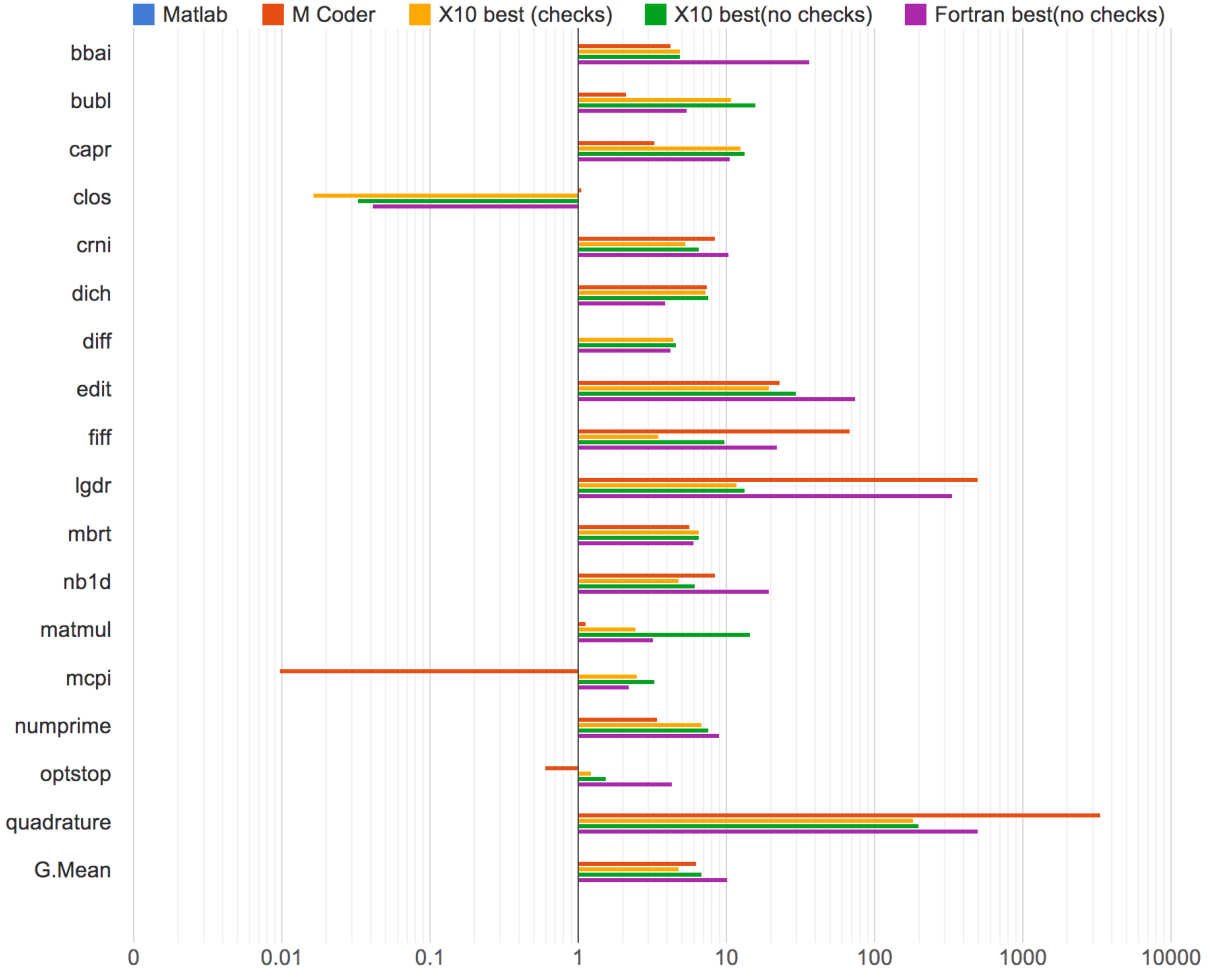
\includegraphics[width=\linewidth]{Figures/final/overall_perf.pdf}
\caption{Performance of \mixten vs other state-of-the-art static
compilers, reported as speedups relative to Mathworks' \matlab,  higher
is better.} \label{Fig:overall_perf} 
\end{center} 
\end{figure*} 

\figref{Fig:overall_perf} shows the speedups and slowdowns for the code
generated for our benchmarks by different compilers.  For \mixten we have
included the results for the \xten code compiled by the \xten C++ backend
compiled, once with \texttt{-NO\_CHECKS} enabled and once with
\texttt{-NO\_CHEKCS} disabled.  For Fortran we included the results for the
code generated without bounds checks.  C code from \matlab coder was generated
with default settings and includes bounds checks. We also calculated the
geometric mean of speedups(slowdowns) for all the benchmarks for each compiler. 

Overall, one can see that the static compilers all provide excellent
speedups, often of at least an order of magnitude faster.  Thus, for the
kinds of benchmarks in our benchmark set, it would seem that tools like
the \matlab coder, \mctwofor, and our \mixten tools are very useful.
\mixten outperforms \matlab coder in 9 out of 17 benchmarks, when
compared with the \xten version compiled with bounds checks, and 10 out
of 17 benchmarks when compared with the version with no bounds checks.
For Fortran, the generated \xten does better in 7 out of 17 benchmarks
with no bounds checks, and 6 out of 17 benchmarks with bounds checks
enabled.  Note that \matlab coder was not able to compile 1 of our
benchmarks (\emph{diff}) due to the dynamic array
growth involved in it; \mixten supports dynamic array growth.  

We achieved a mean speedup of 4.8
over \matlab, for the \xten code with bounds checks, and 6.8 for the x10 code
with no bounds checks.  On the other hand, \matlab coder gave a mean speedup of
6.3 and \mctwofor gave a mean speedup of 10.2.  However, we noticed that our
mean result was skewed due to two benchmarks for which the generated \xten
performed very poorly compared to the generated C code.  These benchmarks are
\emph{clos} and \emph{lgdr}. In the following paragraphs we explain the reason
for their poor performance.  If  we do not consider these two benchmarks, we
get a mean speedup of 6.7 for the \xten code with bounds checks compared to 5.2
for the C code. For the \xten code compiled with no bounds checks we get a mean
speedup of 9.3 compared to 11.6 for Fortran. 

\emph{clos} involves repeated calls to the builtin matrix multiplication
operation for the 2-dimensional matrices. The generated C code from \matlab
coder uses highly optimized matrix multiplication libraries compared to the
naive matrix multiplication implementation used by \mixten. Thus, \mixten gets a
speedup of 0.02 as compared to 1.05 for C. Note that the generated Fortran
code is also slowed down (speedup of 0.04) due to the same reason. As a future
work, We plan to replace our matrix multiplication implementation with calls to
an optimized library function.       

\emph{lgdr} involves repeated transpose of a row vector to a column vector.
\matlab and Fortran, both being array languages are highly optimized for
transpose operations. \mixten currently uses a naive transpose algorithm which
is not optimized. We did achieve a speedup of over 10 times compared to \matlab
but it is not as good as the speedups achieved by C (speedup of 505.0) and
Fortran (speedup of 336.7). For transpose operation also, we plan to replace
our current implementation with an optimized implementation or a call to an
optimized library function.  

Both of these examples show that in addition to generating good code,
another important task is developing optimized \xten library routines for key
array computations.

Other interesting numbers are shown by \emph{optstop},
\emph{fiff}, \emph{nb1d}, and \emph{quadrature}.  \emph{optstop} gave a speedup
of just 1.5 even without bounds checks. It involves repeated random number
generation, which our experiments showed to be slow for the \xten C++ backend
compared to Fortran and even the Java backend.  This problem is worse with C,
due to which the C code from \matlab coder gives a speedup of mere
0.6(slowdown). Fortran performs better with a speedup of 4.3.  \emph{bbai}
shows a similar pattern due to the same reason. 
\begin{comment}
 \emph{numprime} involves a for
loop over a conditional that evaluates to true only once. \matlab coder
leverages this fact for optimizing the for loop by implicitly inserting a
\texttt{break} when the conditional becomes true. C code for \emph{numprime}
provides a speedup of 792.00 compared to 6.83 for \xten and 9.00 for java.  We
tested our generated \xten code by explicitly inserting a \texttt{break}
statement and achieved a speedup of around 65 times. Note that \emph{numprime}
is also used for demonstrating \texttt{parfor} which does not allow a
\texttt{break} statement in the loop.
\end{comment}
\emph{fiff} is characterized by stencil
operations in a loop on a 2-dimensional array. These operations are also
optimized by array-based languages like Fortran and \matlab.  For \emph{nb1d},
Fortran performs better due to the use of column vectors in the benchmark, which
are represented as 2-dimensional arrays in \xten but in Fortran they are
represented as 1-dimensional and are optimized. 2-dimensional arrays are not as
fast in \xten as the 1-dimensional arrays.  \emph{quadrature} involves repeated
arithmetic calculations on a range of numbers. We achieve a speedup of about 200
times compared to \matlab, however it is slow compared to speedups of 3348 and
502 by C and Fortran respectively.  We believe that \matlab coder leverages
partial evaluation for optimizing numerical methods' implementations.

\begin{comment} VK:
 reasoning for quadrature is a speculation. I am not very sure
if this is the case. The program is really simple and there seems to be nothing
unique going on.  
\end{comment}

For most of the other benchmarks, we perform better or nearly equal to C and
Fortran code. Despite the facts that: (1) the sequential core of \xten is a
high-level object oriented language which is not specialized for array-based
operations; and (2) Generating the executable binaries via \mixten involves two
levels of source-to-source compilations (\matlab $\rightarrow$ \xten
$\rightarrow$ C++); we have achieved performance comparable to C, the state of
the art in statically compiled languages and Fortran, a statically compiled
language highly specialized for arrays.
       
\section{\xten C++ Backend vs. \xten Java Backend}

The \xten compiler provides two backends, a C++ backend that compiles the \xten
code to native binary via C++, and a Java backend that compiles the \xten code
to JVM code via Java. We were interested to see how well these backends perform
when used to compile the \mixten generated code. Even though we did not expect
Java code to perform as well as the C++ code, our aim was to make sure that we
achieved good performance, significantly better than \matlab, for the \xten
Java backend.  This would enable \matlab programmers to use our \mixten
compiler to generate code that could be integrated into Java applications. 

In this section we present the performance comparison of the \mixten
generated \xten code compiled by the \xten C++ backend with that compiled by
the \xten Java backend. Columns 3 and 4 of the Table \ref{tab:cpp_vs_java} show
speedups for our benchmarks compiled with the \xten C++ backend without bounds
checks, and with bounds checks respectively. Columns 5 and 6 show these values
for compilation with the \xten Java backend without bounds checks, and with
bounds checks respectively. We also show the geometric mean of the speedups for
all the 4 cases. 

\begin{table*}[htbp]
\begin{center} 
\begin{footnotesize}
\begin{tabular}{|r|c|c c|c c|} \hline Benchmark      & Matlab & C++ (no checks)
& C++ (checks) & Java (no checks) & Java (checks) \\ \hline bbai           & 1
& 4.9             & 4.9          & 11.3             & 10.7          \\ bubl
& 1      & 15.8            & 10.8         & 7.5              & 7.5           \\
capr           & 1      & 13.5            & 12.7         & 11.1             &
6.3           \\ clos           & 1      & 0.03            & 0.02         & 0.02
& 0.002         \\ crni           & 1      & 6.5             & 5.3          &
5.6              & 4             \\ dich           & 1      & 7.6             &
7.3          & 7                & 1.6           \\ diff           & 1      & 4.6
& 4.4          & 0.3              & 0.3           \\ edit           & 1      &
29.7            & 19.4         & 22.1             & 20            \\ fiff
& 1      & 9.8             & 3.5          & 2.1              & 1.4           \\
lgdr           & 1      & 13.5            & 11.9         & 10.6             &
10.6          \\ mbrt           & 1      & 6.5             & 6.5          & 0.3
& 0.3           \\ nb1d           & 1      & 6.2             & 4.8          &
5.5              & 4.1           \\ matmul         & 1      & 14.7            &
2.5          & 1.1              & 0.8           \\ mcpi           & 1      & 3.3
& 2.5          & 2.9              & 3             \\ numprime       & 1      &
7.6             & 6.8          & 6.5              & 6.4           \\ optstop
& 1      & 1.5             & 1.2          & 1.8              & 1.4           \\
quadrature     & 1      & 200.9           & 182.6        & 167.4            &
154.5         \\ \hline Geometric mean & 1      & 6.8             & 4.8
& 3.4              & 2.4           \\ \hline
\end{tabular}

\end{footnotesize}
\caption{\mixten performance comparison : \xten C++ backend vs. \xten
Java backend, speedups relative to Mathworks' \matlab, higher is better} 
\label{tab:cpp_vs_java} 
\end{center} 
\end{table*}

The mean speedups for the C++ backend are 6.8 and 4.8 respectively for the
version with bounds checks switched off, and the version with bounds checks
switched on, whereas for Java backend these values are 3.4 and 2.4
respectively. This is expected, given that C++ is compiled to native binary
while Java is JIT compiled. 

\emph{bbai} and \emph{optstop} are the two exceptions, where Java performs
better than C++.  For \emph{bbai}, both the Java versions gave a speedup of
over 10, whereas for C++, the speedup is under 5 for both the versions. For
\emph{optstop}, the difference is not large, with C++ speedup at 1.5 (1.2 for
the bounds checks version) compared to 1.8 (1.4 for the bounds checks
version) for the Java backend. \emph{bbai} is slower with \xten C++ backend
because it includes repeated calls to the \xten's \texttt{Random.nextDouble()}
function to generate random numbers. We found it to be significantly slower in
the C++ backend compared to the Java backend. We have reported our findings to
the \xten development team and they have validated our findings. \emph{optstop}
is slower for the same reason : It also involves repeated random number
generation. Note that for these two benchmarks, even the C code generated via
\matlab coder is slower than the C++ code, with speedups of 4.2 and 0.6
respectively for \emph{bbai} and \emph{optstop}. 

Other interesting results are for the benchmarks \emph{diff}, \emph{fiff},
\emph{mbrt} and \emph{matmul}. For these benchmarks, results from the Java
backend are significantly slower compared to the C++ backend.  \emph{diff} and
\emph{mbrt} involve operations on complex numbers. In the \xten C++ backend,
complex numbers are stored as \texttt{structs} and are kept on the stack,
whereas in the Java backend, they are stored as \emph{objects} and reside in
the heap storage.  \emph{fiff} and \emph{matmul}  are characterized by repeated
array access and read/write operations on 2-dimensional arrays.  For these
benchmarks, the Java backend performs significantly slower compared to the C++
backend with no bounds checks(2.1 vs. 9.8 for \emph{fiff} and 1.1 vs.  14.7
for \emph{matmul}), however compared to the performance by the C++ beckend with
bounds checks, it is not as slow(2.1 vs. 3.5 for \emph{fiff} and 1.1 vs.
2.5 for \emph{matmul}).  The reason is that even with bounds checks turned off
for the \xten to Java compiler, The Java compiler by default has bounds checks
on. These checks have a significant effect on performance for 2-dimensional
array operations.

\subsection{When not to use the \xten \texttt{-O}}
\label{sec:BOOM}

One of the most surprising results in this set of experiments was the fact that
we had to sometimes disable the \xten \texttt{-O} optimizer switch when
using the \xten Java backend..
For the benchmarks \emph{capr} and
\emph{dich}, in the case when \xten bounds checks are switched on, we found
very pathological performance, with slowdowns of over 2 orders of magntitude,
when the \xten compiler's optimization switch(\texttt{-O}) was used.

We recorded running times of 785.3 seconds for \emph{capr} compared to 3.2
seconds without the optimization, and 1558.9 seconds for \emph{dich} compared to
12.7 seconds without the optimization.  With the help of the \xten development
team we determined that switching on the optimization triggered code inlining
for the array bounds check code, which then
caused the resultant Java program to be too large to be handled by the JIT
compiler.  In fact, the Java JIT effectively gives up on this code and reverts 
to the interpreter. 

Thus, it would seem that the \xten optimizer needs to be improved in order to
apply aggressive inlining only when it does not have a negative impact on code
size,  and that different inlining strategies are needed for the C++ and Java
backends.

\section{Simple vs. Region Arrays} \label{sec:EvalArrays}

One of the key optimizations used by \mixten is to use simple arrays,
wherever possible, for higher performance.  In this section we discuss the
performance gains obtained by using simple arrays over region arrays and
the specialized region arrays.  A description of these three kinds of arrays
provided by \xten was given in \secref{subsec:ArrayDesc}.  Table
\ref{tab:simple_vs_region} shows the relative speedups and slowdowns for our
benchmarks compiled to use different kinds of \xten arrays for the C++ backend
and the Java backend.

\begin{table*}[htbp]
\begin{center} 
%\begin{footnotesize}
\scalebox{0.67}{
\begin{tabular}{|r|c|ccc|ccc|}
\hline
           &        & \multicolumn{3}{c|}{X10 C++ backend}                   &
\multicolumn{3}{c|}{X10 Java backend}                  \\ \hline
Benchmark  & Matlab & Simple arrays & Region arrays & Special region arrays &
Simple arrays & Region arrays & Special region arrays \\ \hline
bbai           & 1.0     & 4.9                    & 2.7                     & 2.7                             & 11.3                         & 6.4                      & 6.6                              \\
bubl           & 1.0     & 15.8                   & 11.4                    & 11.6                            & 7.5                          & 3.6                      & 3.7                              \\
capr           & 1.0     & 13.5                   & 11.6                    & 12.4                            & 11.1                         & 0.02                        & 10.5                             \\
clos           & 1.0     & 0.03                   & 0.01                    & 0.01                               & 0.02                         & 0.01                     & 0.01                             \\
crni           & 1.0     & 6.5                    & 3.6                     & 3.9                             & 5.6                          & 4                        & 4.1                              \\
dich           & 1.0     & 7.6                    & 6.7                     & 7.0                               & 7.0                            & 0.01                        & 0.02                                \\
diff           & 1.0     & 4.6                    & 4.2                     & 4.3                             & 0.3                          & 0.3                      & 0.3                              \\
edit           & 1.0     & 29.7                   & 4.3                     & 3.6                             & 22.1                         & 9.4                      & 9.4                              \\
fiff           & 1.0     & 9.8                    & 2.0                       & 2.8                             & 2.1                          & 1.4                      & 1.4                              \\
lgdr           & 1.0     & 13.5                   & 1.6                     & 1.5                             & 10.6                         & 5.4                      & 5.4                              \\
mbrt           & 1.0     & 6.5                    & 6.3                     & 6.5                             & 0.3                          & 5.1                      & 5.1                              \\
nb1d           & 1.0     & 6.2                    & 0.3                     & 0.3                             & 5.5                          & 1.4                      & 1.4                              \\
matmul         & 1.0     & 14.7                   & 1.3                     & 1.4                             & 1.1                          & 0.5                      & 0.5                              \\
mcpi           & 1.0     & 3.3                    & 2.8                     & 2.7                             & 2.9                          & 3.0                        & 3.0                                \\
numprime       & 1.0     & 7.6                    & 5.7                     & 5.7                             & 6.5                          & 6.3                      & 6.3                              \\
optstop        & 1.0     & 1.5                    & 0.4                     & 0.4                             & 1.8                          & 1.2                      & 1.3                              \\
quadrature     & 1.0     & 200.9                  & 200.9                   & 200.9                           & 167.4                        & 143.5                    & 154.5                            \\ \hline
Geometric mean & 1.0     & 6.8                    & 2.7                     & 2.8                             & 3.4                          & 1.3                      & 1.9  
\\ \hline                           
\end{tabular}

}
%\end{footnotesize}
\caption{\mixten performance comparison : Simple
arrays vs. Region arrays vs.  Specialized region arrays, speedup relative to 
Mathworks' \matlab, higher is better} 
\label{tab:simple_vs_region} 
\end{center}
\end{table*}

For the C++ backend we obtained a mean speedup of 6.8 for Simple arrays,
compared to 2.7 for region arrays and 2.8 for specialized region arrays. For
the Java backend, we obtained speedups of 3.4, 1.3 and 1.9 for the simple
arrays, region arrays, and the specialized region arrays respectively. These
results are as expected in \secref{Sec:CompileArrays}. For the C++ backend,
most noticeable performance differences between simple arrays and region arrays
are for \emph{edit}, \emph{fiff}, \emph{lgdr}, \emph{nb1d}, \emph{matmul} and
\emph{optstop}. All of these benchmarks are characterized by large number of
array accesses and read/write operations on 2-dimensional arrays, except
\emph{optstop} and \emph{edit}, which have multiple large 1-dimensional arrays.
The performance difference is most noticeable for \emph{nb1d}, where the region
arrays are about 20 times slower than the simple arrays. This is because
\emph{nb1d} involves simple operations on a large column vector. With simple
arrays, since the compiler knows that it is a column vector, rather than a
2-dimensional matrix, even though it is declared as a 2-dimensional array, the
performance can be optimized to match that of the underlying \texttt{Rail}.
However, this is not possible for region arrays where the size of each
dimension is not known statically. For the C++ backend, we do not observe
significant performance differences between the region arrays and the
specialized region arrays.

For the Java backend we observed a higher difference in the mean performance
for the simple arrays and the region arrays. The mean speedup for region arrays
is 1.3 whereas for simple arrays it is nearly 3 times more at 3.4. There is
also a significant difference between the performance of specialized region
arrays and region arrays. Speedup for specialized region arrays is 1.9. Like
the C++ backend, here also, most noticeable performance gain for simple arrays
is for benchmarks involving a large number of array accesses and read/writes.
\emph{capr} and \emph{dich} ask for special consideration. For \emph{capr},
even with \xten compiler's bounds checks turned off, the region array version
slows down by more than 500 times compared to the simple array version and even
the specialized region array version. This again, is due to the fact that
region arrays, with the dynamic shape checks, generated more code than the JIT
compiler could handle. For \emph{dich} the slowdown due to region arrays was
about 700 times compared to simple arrays. For \emph{dich}, even the
specialization on region arrays was not enough to reduce the code size enough
to be able to be JIT compiled. 

\section{Effect of the IntegerOkay Analysis}    
\label{sec:intok_perf}

In this section we present an overview of the performance improvements
achieved by \mixten by using the IntegerOkay analysis. Table \ref{tab:int_vs_double}
shows a comparison of speedups gained by using the IntegerOkay analysis over
those without using it. For this experiment we used results with \xten
optimizations turned on and bounds checks turned off. 
   
\begin{table*}[htbp]
\begin{center} 
\begin{footnotesize}
\begin{tabular}{|r|c|cc|cc|}
\hline
               &        & \multicolumn{2}{c|}{X10 C++ backend} &
\multicolumn{2}{c|}{X10 Java backend} \\ \hline
Benchmark      & Matlab & IntegerOkay      & All Doubles      & IntegerOkay
& All Doubles      \\ \hline
bbai       & 1.0    & 4.9             & 3.8                & 11.3                         & 8.2                 \\
bubl       & 1.0    & 15.8            & 2.2                & 7.5                          & 4.2                 \\
capr       & 1.0    & 13.5            & 1.7                & 11.1                         & 9.7                 \\
clos       & 1.0    & 0.03            & 0.02               & 0.02                         & 0.01                \\
crni       & 1.0    & 6.5             & 2.8                & 5.6                          & 5.5                 \\
dich       & 1.0    & 7.6             & 1.0                & 7.0                          & 5.8                 \\
diff       & 1.0    & 4.6             & 4.5                & 0.3                          & 0.3                 \\
edit       & 1.0    & 29.7            & 13.5               & 22.1                         & 20.0                \\
fiff       & 1.0    & 9.8             & 1.0                & 2.1                          & 1.8                 \\
lgdr       & 1.0    & 13.5            & 10.1               & 10.6                         & 11.0                \\
mbrt       & 1.0    & 6.5             & 6.1                & 0.3                          & 0.3                 \\
nb1d       & 1.0    & 6.2             & 5.2                & 5.5                          & 5.5                 \\
matmul     & 1.0    & 14.7            & 14.5               & 1.1                          & 1.2                 \\
mcpi       & 1.0    & 3.3             & 3.3                & 2.9                          & 2.9                 \\
numprime   & 1.0    & 7.6             & 7.6                & 6.5                          & 7.1                 \\
optstop    & 1.0    & 1.5             & 1.0                & 1.8                          & 1.0                 \\
quadrature & 1.0    & 200.9           & 182.6              & 167.4                        & 143.5               \\ \hline
Geometric mean         & 1.0    & 6.8             & 3.4                & 3.4                          & 2.9                 \\ \hline
\end{tabular}

\end{footnotesize}
\caption{Performance evaluation for the IntegerOkay
analysis, speedups relative to Mathworks' \matlab, higher is better} 
\label{tab:int_vs_double} 
\end{center} 
\end{table*}

For the C++ backend, we observed a mean speedup of 6.8 which is two
times the speedup gained by not using the IntegerOkay analysis, which is equal
to 3.4. We observed a significant gain in performance by using IntegerOkay
analysis for the benchmarks that involve significant number of array indexing
operations. \emph{bubl}, \emph{capr}, \emph{crni}, \emph{dich}, and \emph{fiff} 
show the most significant performance gains. The reason for this
behaviour is that, \xten requires all array indices to be of type \texttt{Long},
thus if the variables used as array indices are declared to be of type
\texttt{Double} (which is the default in \matlab), they must be typecast to
\texttt{Long} type. \texttt{Double} to \texttt{Long} is very time consuming
because every cast involves a check on the value of the \texttt{Double} type
variable to ensure that it can safely fit into \texttt{Long} type. 

For the Java backend, with the IntegerOkay analysis, we get a mean speedup of
3.4 as compared to 2.9 without it. The reason for the lower difference as
compared to that for the C++ backend is that, for Java backend, the \xten
compiler does not generate the value checks for \texttt{Double} type values,
instead it relies on the JVM to make  these checks, resulting in a better
performance.  Also note that, without the IntegerOkay analysis, the C++ backend
results are slower than the Java backend results for 9 out of 17 benchmarks.

To conclude, IntegerOkay analysis is very important for efficient performance of
code involving Arrays, specially for the \xten C++ backend.

\section{\matlab parfor vs. \mixten Parallel Code}
\label{sec:parfor_results}
 
Given that we have established that we can generate competitive
sequential code, we wanted to also do a preliminary study to see if we
could get additional benefits from the high-perfomance nature of \xten.
In this section we present the preliminary results for the
compilation of \matlab \texttt{parfor} construct to the parallel \xten
code. 7 out of our 17 benchmarks could be safely modified to use the
\texttt{parfor} loop.  We compare the performance of the generated
parallel \xten programs for these benchmarks to that of \matlab code
using \texttt{parfor}, and to their sequential \xten versions. For this
experiment, we used the sequential versions of the generated \xten
programs with optimizations and no bounds checks.  For the parallel
versions we used both the variants, with optimizations and bounds
checks, and with optimizations and without bounds checks.  Table
\ref{tab:parfor_vs_x10} shows the results for both the \xten C++ and the
\xten Java backends.
   
\begin{table*}[htbp]
\begin{center} 
%\begin{footnotesize}
\scalebox{0.7}{
\begin{tabular}{|r|c|c|c|cc|c|cc|}
\hline
               &        &               & \multicolumn{3}{c|}{X10 C++ backend}
& \multicolumn{3}{c|}{X10 Java backend}          \\ \hline
               &        &               & Sequential &
\multicolumn{2}{c|}{Parallel}     & Sequential & \multicolumn{2}{c|}{Parallel}
\\ \hline
Benchmarks     & MATLAB & MATLAB parfor &   No checks & No checks & 
Checks &     No checks       & No checks & Checks \\ \hline
mbrt           & 1.0    & 1.7           & 6.5                            & 25.3                         & 25.3                      & 0.3                             & 1.3                           & 1.3                        \\
nb1d           & 1.0    & 0.4           & 6.2                            & 7.3                          & 7.3                       & 5.5                             & 19.0                          & 15.1                       \\
matmul         & 1.0    & 1.3           & 14.7                           &
68.7                        & 3.9                       & 1.1                             & 1.1                           & 0.8                        \\
mcpi           & 1.0    & 4.6           & 3.3                            & 15.7                         & 15.9                      & 2.9                             & 18.1                          & 18.2                       \\
numprime       & 1.0    & 5.3           & 7.6                            & 30.0                         & 30.9                      & 6.5                             & 24.8                          & 26.4                       \\
optstop        & 1.0    & 4.1           & 1.4                            & 2.0                          & 2.1                       & 1.8                             & 10.7                          & 9.7                        \\
quadrature     & 1.0    & 3.8           & 200.9                          & 11.3                         & 11.2                      & 167.4                           & 13.0                          & 13.0                       \\ \hline
Geometric mean & 1.0    & 2.3           & 8.9                            &
14.5                         & 9.8                       & 3.7                             & 7.8                           & 7.1                        \\ \hline
\end{tabular}
 
%\end{footnotesize}
}
\caption{Performance evaluation for \mixten generated
parallel \xten code for the \matlab \texttt{parfor} construct, speedups
relative to Mathworks' \matlab,  higher is better} 
\label{tab:parfor_vs_x10} 
\end{center} 
\end{table*}

For the \xten C++ backend we achieved a mean speedup of 16.0 for the
generated parallel \xten code without bounds checks, which is over 9
times of the speedup for the \matlab code with \texttt{parfor}, at a
speedup of 2.3. Compared to \xten sequential code which has a mean
speedup of 8.9, it is nearly twice as fast.  Even with the parallel
\xten code with bounds checks we achieved a speedup of 9.8 which is over 4
times better than the \matlab \texttt{parfor} code.  \emph{optstop} is
an interesting exception. It is actually slower (at a speedup of 2.1)
than the \matlab \texttt{parfor} version (at a speedup of 4.1). The
sequential version of \emph{optstop} is just slightly faster than the
sequential \matlab version, with a speedup of just 1.5 (due to the
reasons explained earlier) and the total time for the parallel execution
of each iteration, and managing the parallelization of these activities
is just slightly faster than the sequential version. We see a similar
trend for the \emph{matmul} benchmark for the \xten Java backend. It
shows a speedup of just 0.8 (version with bounds checks) as compared to
1.3 for the \matlab \texttt{parfor} version. Overall, for the Java
backend we obtained a mean speedup of 7.8 for the \xten code with no
bounds checks and 7.1 for the code with bounds checks. Compared to the
\matlab parfor version we obtained about 3.5 times better performance. The
parallel \xten code is over 2 times faster than the sequential \xten
code (speedup of 3.7).For both, the C++ backend, and the Java backend,
the mean speedup for the sequential \xten code is also substantially
faster than the \matlab parallel code.  

To conclude, the parallel \xten code provides much higher performance
gains compared to the \matlab \texttt{parfor} code  and even the \xten
sequential code, which by itself is most of the times faster than the
\matlab parallel code.


\section{Summary}

We showed that the \mixten compiler with its efficient handling of array
operations and optimizations like IntegerOkay can generate \xten code
that provides performance comparable to the native code generated by the
state of the art languages like C, which is fairly low-level, and
Fortran, which itself is an array-based language.  As a future work, we
plan to use more efficient implementations of the builtin functions, and
believe that it would further improve the performance of the code
generated by \mixten.

With \mixten, we also took first steps to compile \matlab to parallel
\xten code to take full advantage of the high performance features of
\xten. Our preliminary results are very inspiring and we plan to
continue in this direction further, in the future.

In addition to demonstrating that our approach leads to good code, these
experiments have also been quite valuable for the \xten development team.
Our generated code has stressed the \xten system more than the
hand-written \xten benchmarks and has exposed places where further
improvements can be made.
